\documentclass[11pt,a4paper]{article}

\usepackage[utf8]{inputenc}
\usepackage[english]{babel}
\usepackage[T1]{fontenc}

\usepackage{amsmath,amssymb,amsfonts}

\usepackage{hyperref}
\usepackage{graphicx}

\title{Statistical Methods for Machine Learning - Exam}
\author{Sebastian Paaske Tørholm}

\begin{document}
\maketitle

\section{General comments}
The code is written in MATLAB R2012b, and makes use of the built-in library functions.

\section{Sunspot Prediction}
For question 1, I have chosen to use a maximum likelihood estimate, with a
linear design matrix. I do not use a built-in implementation.

The maximum likelihood model found is defined by the following weight vector:

\[
    \mathbf{w}_{ML} = \begin{pmatrix} 10.844 \\ -0.062 \\ 0.121 \\ -0.012 \\ -0.570 \\ 1.284 \end{pmatrix}
\]


For question 2, I use MATLAB's built in neural network implementation for
this. I've chosen to use a feed-forward neural network with 5, 10 and 15
hidden neurons. The network is trained using the RProp algorithm described at
the lectures.

The implementation makes use of regularization and early stopping to improve
the generalization performance and help reduce overfitting.

\begin{figure}[h!]
    \centering
    \begin{tabular}{|l|l|l|}
        \hline
        Model & RMS (training data) & RMS (testing data) \\
        \hline
        Linear ML & 14.067 & 18.770 \\
        NN (5 hidden neurons) & 13.390 & 19.695 \\
        NN (10 hidden neurons) & 13.210 & 21.924 \\
        NN (15 hidden neurons) & 12.902 & 24.196 \\ 
        \hline
    \end{tabular}
    \label{sunspots-rms}
    \caption{RMS of the sunspot predictions.}
\end{figure}

In \autoref{sunspots-rms}, we see that the neural networks provide a better
prediction on the training data, but that the linear model wins on the testing
data. This could be due to the neural network overfitting itself to the
training data, and we in fact see that the fewer neurons we use, the better
the RMS is on the testing data.

One could suspect that given the good performance on the linear model, a model
with shortcuts may provide a better performance for the neural network, as it
could introduce more linearity.

\begin{figure}[h!]
    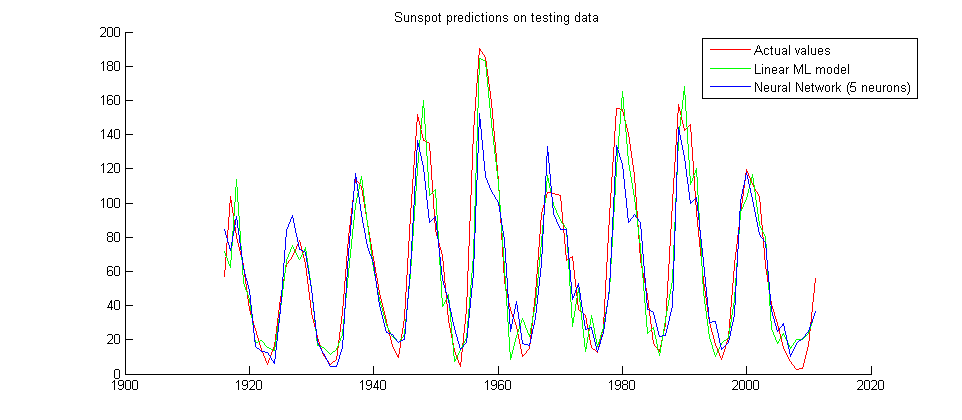
\includegraphics[width=\textwidth]{images/sunspots-testing.png}

    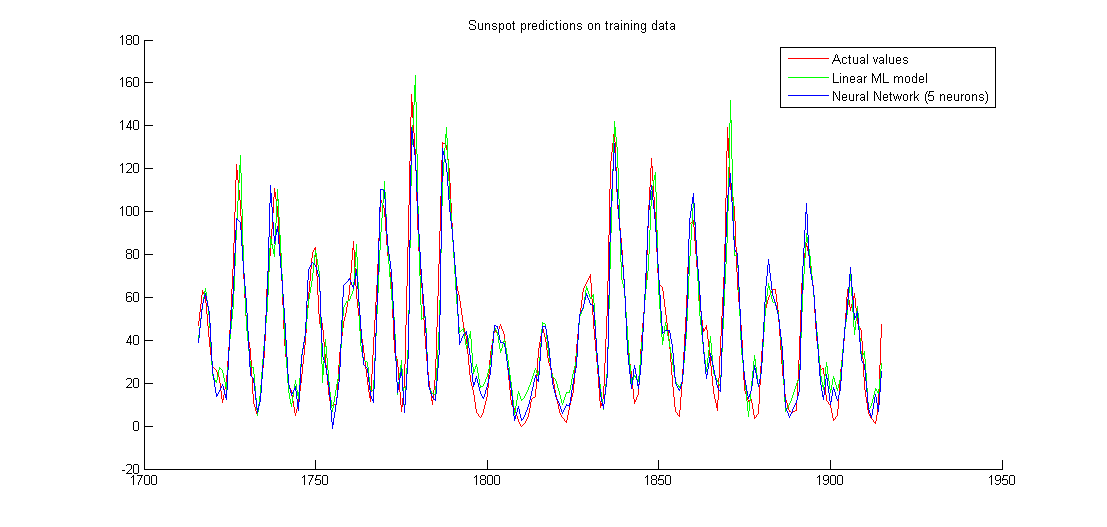
\includegraphics[width=\textwidth]{images/sunspots-training.png}
    \caption{Plots of the predictions on the sunspot testing and training data.}
    \label{sunspots-plots}
\end{figure}

In \autoref{sunspots-plots} we see the predictions plotted against the actual
expected number of sunspots. The linear model does seem to follow the data
more closely, explaining the lower RMS. Especially around 1960, the large
number of sunspots isn't sufficiently modelled by the NN model, whereas the
linear model captures it.

\section{Question 4}
$\sigma_{\text{Jaakkola}}$ was computed by dividing the dataset into stars
and quasars, followed by finding the median as described. This gives
$\sigma_{\text{Jaakkola}} = 3.907$.

For the grid search, I've chosen to use $b = e$ as the base number. Instead of
computing $\gamma_{\text{Jaakkola}}$, I make use of

\[
    \sigma_{\text{Jaakkola}} \cdot b^{-i/2} = \sqrt{1/(2 \gamma_{\text{Jaakkola}} b^i)}
\]

I use the built-in SVM functionality for MATLAB as my SVM implementation. The
data for the SVM is automatically normalized by the implementation, improving
SVM performance, as we saw in assignment 3.

The grid search yielded

\[ \sigma = \sigma_{\text{Jakkola}} \cdot e^{-3/2} = 0.872 \quad\quad C = e^3 = 20.086 \]

as optimal hyperparameters. Using these hyperparameters yields the 0-1 correct rates shown in
\autoref{star-correctrates}. 

\begin{figure}[h!]
    \centering
    \begin{tabular}{|l|l|}
        \hline
        Data set & 0-1 correct rate \\
        \hline
        Testing set & $97.87\%$ \\
        Training set & $98.64\%$ \\
        \hline
    \end{tabular}
    \label{star-correctrates}
    \caption{0-1 correct rates for the SVM with optimal hyperparameters.}
\end{figure}

\section{Question 5}


\section{Question 6}


\section{Question 7}


\section{Question 8}


\end{document}

